% Please give the surname of the lead author for the running footer
\leadauthor{D'Amico, Gabbolini, Parroni}

\title{Robust background subtraction in traffic environments}
%NM-BC: The title is limited to 10 words (or 90 characters)
\shorttitle{Background subtraction}

% Use letters for affiliations, numbers to show equal authorship (if applicable) and to indicate the corresponding author
\author[1 \space *]{D'Amico Edoardo}
\author[1 \space *]{Gabbolini Giovanni}
\author[1 \space *]{Parroni Federico}

\affil[1]{Politecnico di Milano, IT}
\affil[*]{These authors contributed equally.}

\maketitle

\section*{Abstract}
\begin{abstract}
In this paper we present a method for background subtraction with the aim to work on a 24/24h videos
scenario, real time, robust to weather changes and capable to keep foreground objects detected for a
large amount of time. The work is the base to implement a monitoring system for dangerous event in
the road (possible scenario is the monitoring system on highways). The system can be expanded to
detect events such as car driving in the wrong direction, car accidents or people crossing the road.
The model studied is the PBAS (Pixel-Based Adaptive Segmenter): it follows a parametric background
modeling paradigm, thus the background is modeled by a history of recently observed pixel values.
The foreground decision depends on a decision threshold. The background update is based on a learning
parameter. Both parameters are extended to dynamic per-pixel state variables and introduce dynamic
controllers for each of them. Furthermore, both controllers are steered by an estimate of the background
dynamics. All the hyperparameters of the models have been studied and tuned minutely to accomplish the
aimed task.
\end {abstract}

\begin{keywords}
    Background subtraction | Foreground detection | PBAS algorithm | Car | Traffic | Road | Highway | Surveillance |
    Stationary camera | Image processing and analysis
\end{keywords}


\section*{Introduction}
Background subtraction and foreground detection are the basic tasks of many real application systems,
for example, surveillance systems, autonomous vehicles, semantic image analysis. Background subtraction
consists in finding a category for every pixel in a single or (like in this case) in a frames sequence
of a video and saying if that pixels are part of background or foreground. At the end, the algorithm take as
as input a video and output a binary mask, where 1s are foreground pixels and 0 background pixels.
We restricted our domain to traffic monitoring, in particular this work should put the basis for an automated
tool to identify cars and detect anomalies in highways and roads 24/24h (e.g. car accidents,
traffic jam, wrong-direction driving) using a standard RGB stationary camera.
Critical aspects that must be taken into account while developing such algorithm are a lot, first of all,
variable and bad weather conditions and illumination changes. In fact, it is very hard to distinguish
moving objects in presence of heavy rain, fog or snow. Also during night the environmental situation varies
a lot from the day and our algorithm has to adapt continuosly due to this facts. 
Other problems that we faced are shadows and intermittent object motion.
From the majority of the current algorithms, shadows are treated as foreground because they move along with
objects; a little number of them adopts a 3-class classification (background, foreground, shadow). We
decided to provide a binary classification, considering shadows as part of the background. With regards to
the latter problem, here the challenge is to correctly detect an initially stationary object that begins to
move or when an object that was static starts moving again. We fine-tuned some parameters to make sure
that a moving car that stops after a while will be classified as foreground for a long time before turning
into background, while the opposite event (from static to moving) is easier to handle.
The entire algorithm has been implemented in C++, since compiled code performances are fundamental to
allow the system to work in real-time. In \cite{pbas_and_scene_analysis_fpga}, we can find an integration of
the basic algorithm in a FPGA device, which exploit and hardware implementation to reduce a lot the
computational time.


\section*{Related work}
Over the recent past, a multitude of algorithms and methods for background modeling have been developed.
One of the most prominent and most widely used methods are those based on Gaussian Mixture Models (GMM)
\cite{gmm}. Here, each pixels is modeled as a mixture of weighted Gaussian distributions. Pixels, which
are detected as background are used to improve the Gaussian mixtures by an iterative update rule. A very
important non-parametric method is the ViBe \cite{vibe}. Each pixel in the background model is defined by
a history of the N most recent image values at each pixel and uses a random scheme to update them.
More over, updated pixels can ”diffuse” their current pixel value into neighboring pixel using another
random selection method. The preceding scheme is very similar to the approach followed by the PBAS algorithm.
It can be categorized as a non-parametric method, since it uses a history of N image values as the background
model, and uses a random update rule similar to the one used by the ViBe algorithm. However, in Vibe, the
randomness parameters as well as the decision threshold are fixed for all pixels. In contrast, in the PBAS
algorithm these values are not treated as parameters, but instead as adaptive state variables, which can
dynamically change over time for each pixel separately.


\section*{Proposed approach}


\section*{Experiments}
In this section we first report the results obtained by varying the main model parameters. We also include the
adopted settings that perform best in our scenario. Then, we show some real-case usages of the algorithm,
comparing the different environmental conditions that we found in 24/24h live videos.

\subsection*{N}
$N$ represents how many matrices are kept in memory to model the background.
Each of them stores the history of pixels values.
The greater, the more complex background can be handled but at the cost of heavier
computation. At $N=35$, experimental results show that performance saturates.
\begin{figure*}[!t]
\centering
\subfloat[][N = 2]{
    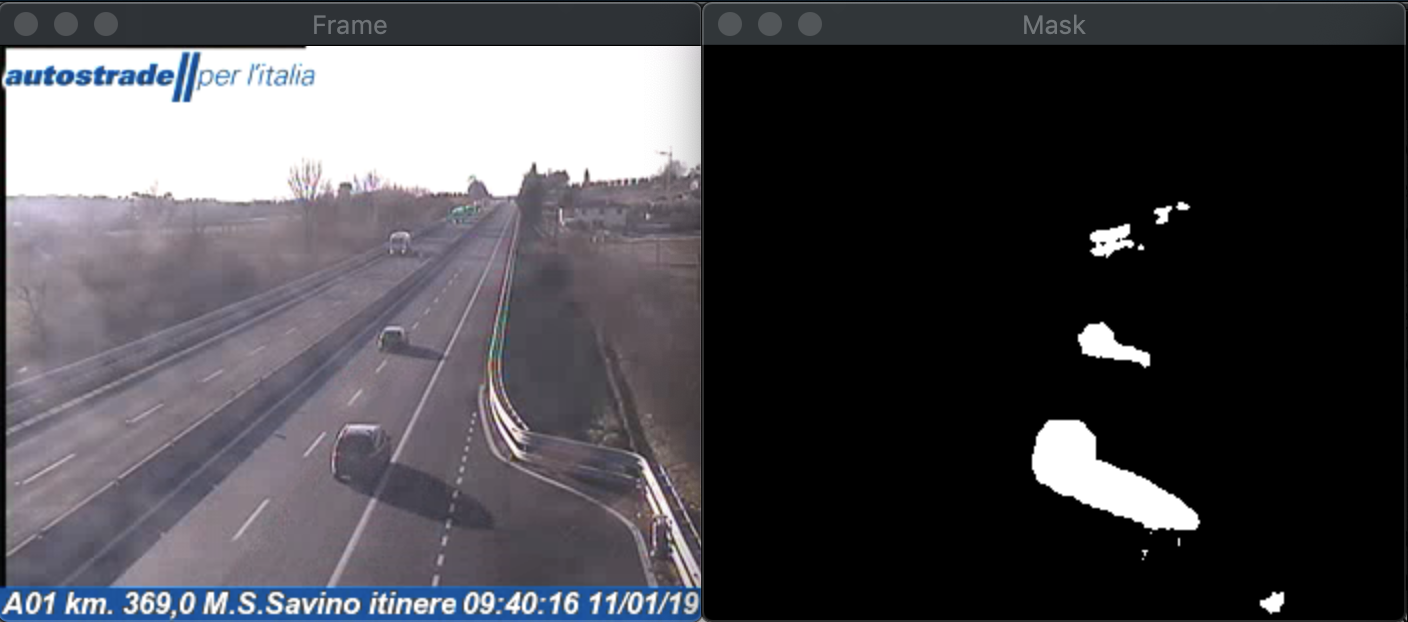
\includegraphics[width=0.32\textwidth]{Figures/N2.jpg}
    %\label{fig:N2}
}
\subfloat[][N = 10]{
    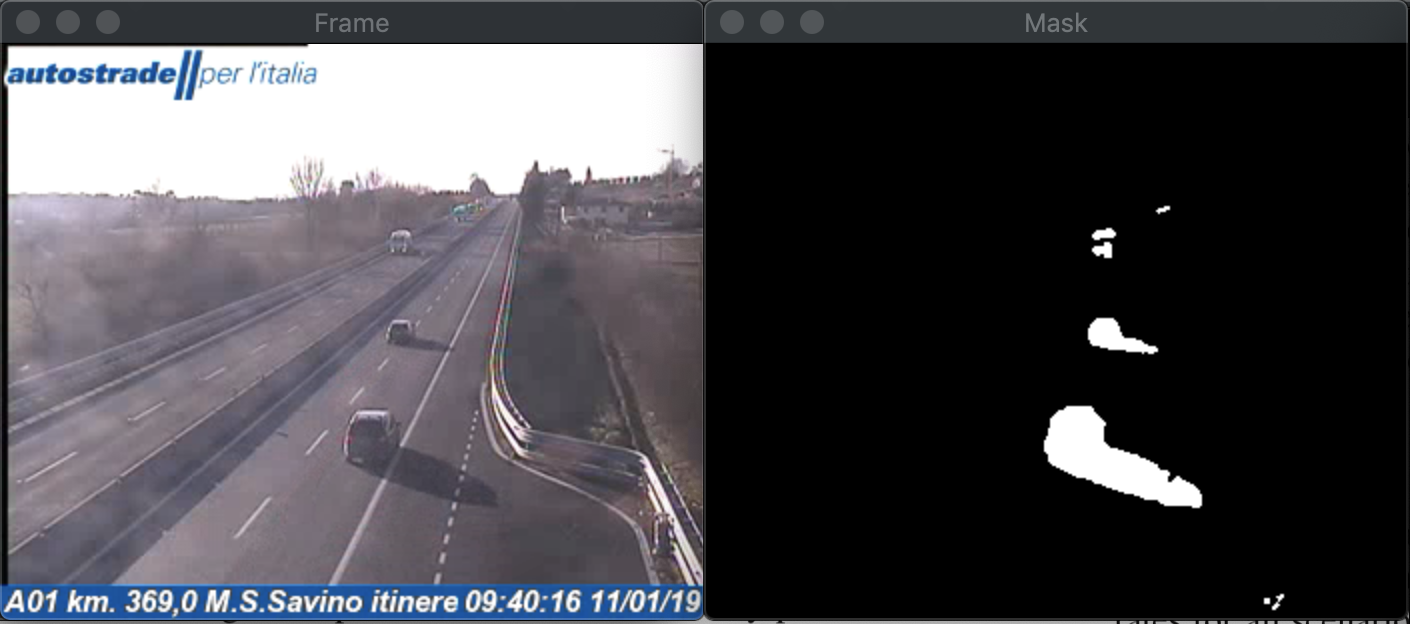
\includegraphics[width=0.32\textwidth]{Figures/N10.jpg}
}
\subfloat[][N = 20]{
    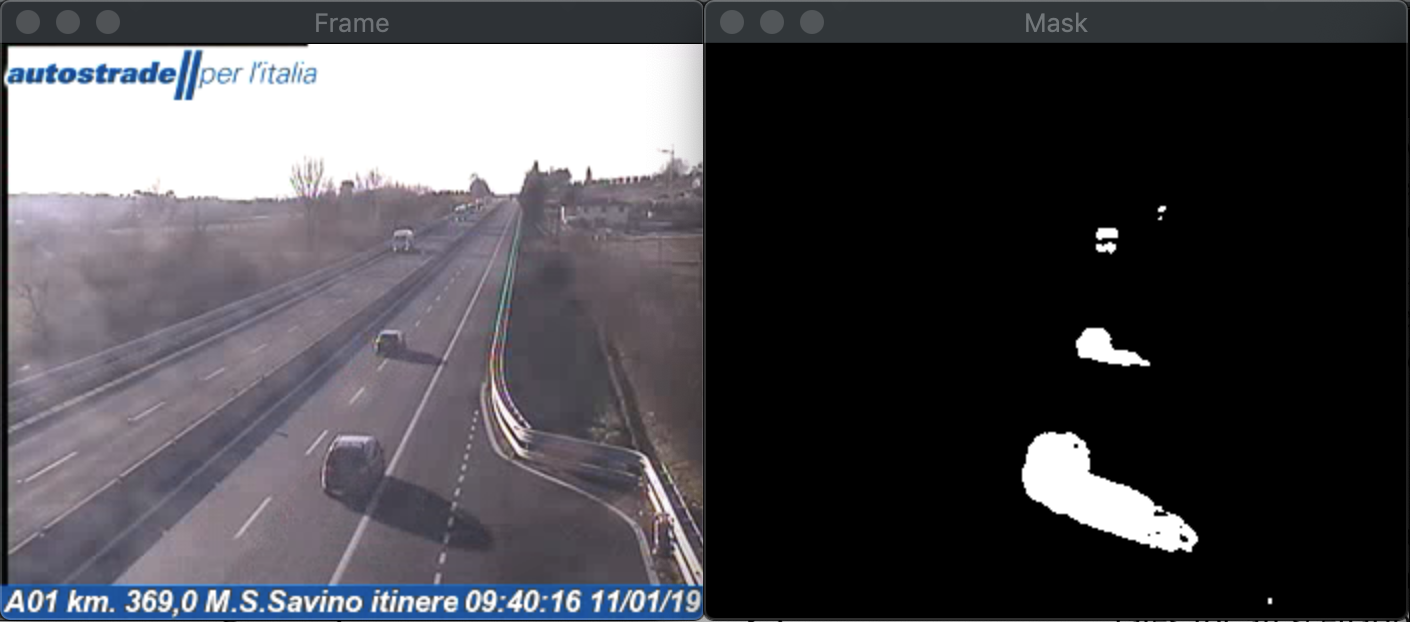
\includegraphics[width=0.32\textwidth]{Figures/N20.jpg}
}
\end{figure*}
We can see the poor mask of the cars on the left road when $N=2$, and the
accurate mask of the lines on the front right when $N=20$.


\subsection*{K}
$K$ tells the number of samples from $B$ that have to be closer than $R$ in order to
classify the pixel as background. The higher, the more difficult for a pixel to be
classified as background.
\begin{figure*}[!t]
\centering
\subfloat[][K = 1]{
    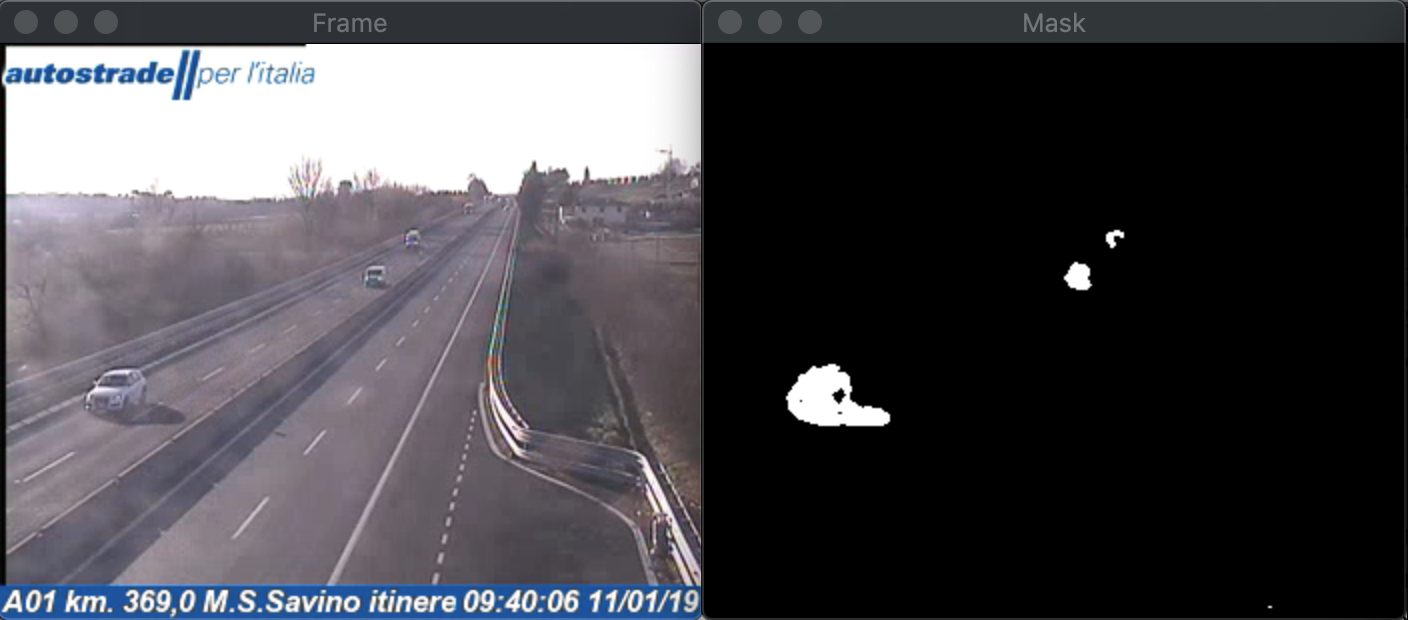
\includegraphics[width=0.32\textwidth]{Figures/K1.jpg}
}
\subfloat[][K = 2]{
    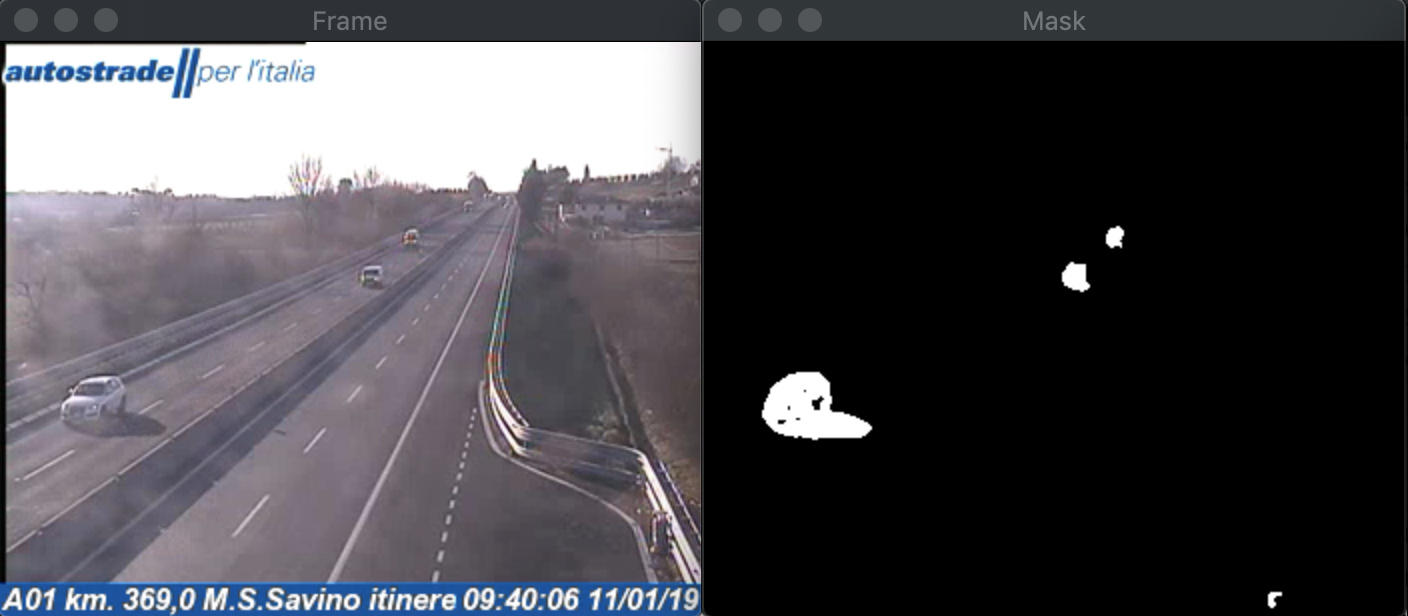
\includegraphics[width=0.32\textwidth]{Figures/K2.jpg}
}
\subfloat[][K = 4]{
    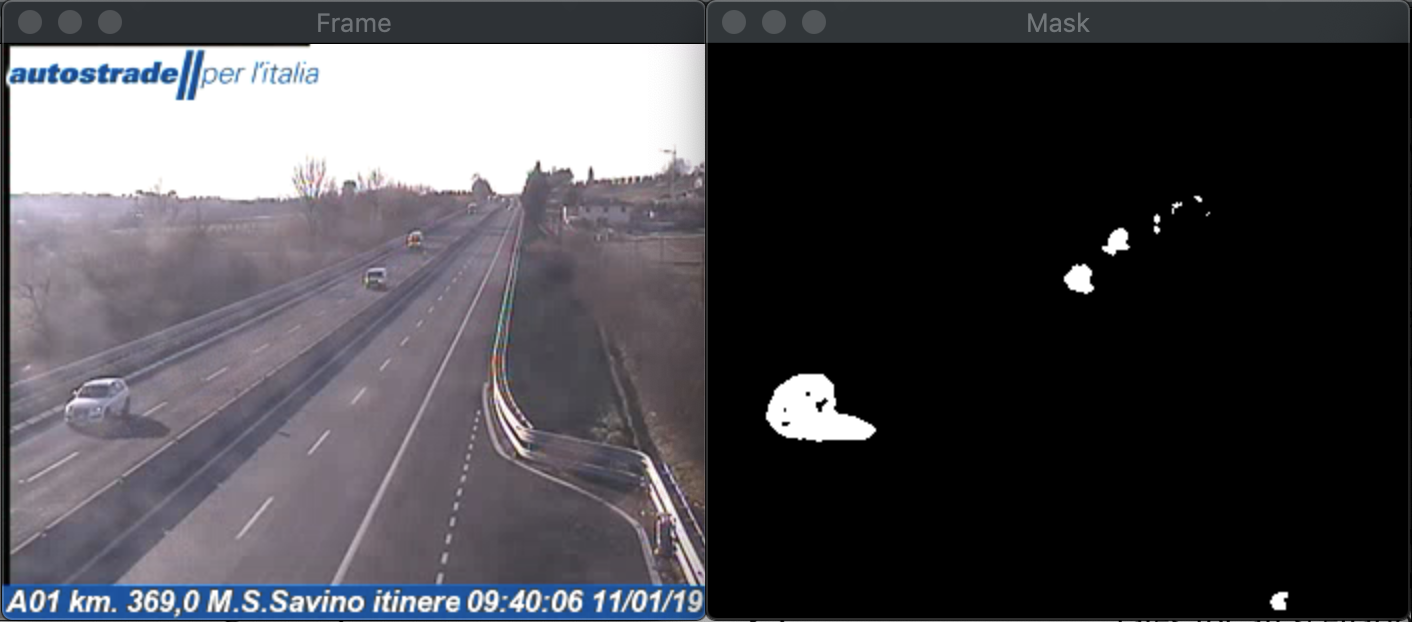
\includegraphics[width=0.32\textwidth]{Figures/K4.jpg}
}
\end{figure*}
We can notice that setting $K$ too high brings to classify many pixels as foreground.

\subsection*{T max}
$T_max$ controls the lowest probability of updating a pixel and putting it the
background model $B$.


\subsection*{R}
Eq ?????????? is similar to the equation of a pure proportional controller.
In this case the $R(x,y)$ has to follow $d_minavg(x,y) * R_scale$. So:
\begin{itemize}
    \item $R_{incdec}$: setting too high lead to oscillation around the target and if
    set too high leads to divergence. The default value is 0.05 which leads to fast
    enough adaptation to the target value (in more or less 30 frames the target is
    reached). Assuming that the backgroud isnt changing much there is no reason to
    raise it.
    \item $R_{scale}$: tells how much the algorithm is sensitive, in fact it is a direct
    control of the threshold. Setting too high it leads to really few false positives
    but also decreases true positives; setting too low, will increase false positives.
    \item $R_{lower}$: sets a limit on how much $R$ can decrease its value. Setting too
    low, it will lead to a lot of false positives in area that are foreground,
    especially if the video is noise, so especially is zones that are clearly
    background are changing their values of high amounts due to noise. Setting too
    high it will reduce true positives. So the choice of it should be lead by the
    video quality, more than the application domain.
\end{itemize}
\begin{figure*}[!t]
    \centering
    \subfloat[][$R_{scale}$ = 5]{
        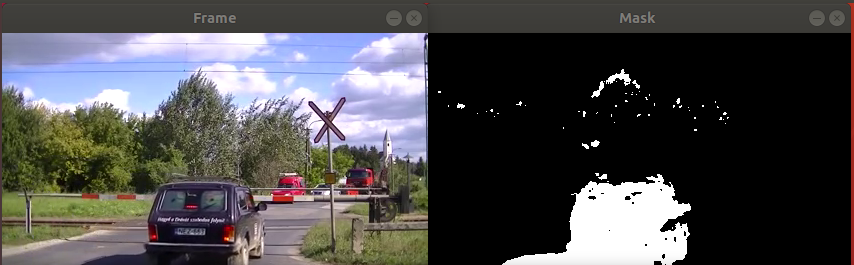
\includegraphics[width=0.32\textwidth]{Figures/R_scale5.jpg}
    }
    \subfloat[][$R_{scale}$ = 15]{
        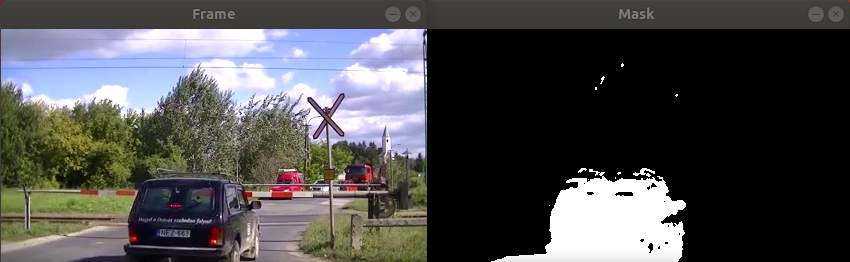
\includegraphics[width=0.32\textwidth]{Figures/R_scale15.jpg}
    }
    \subfloat[][$R_{scale}$ = 50]{
        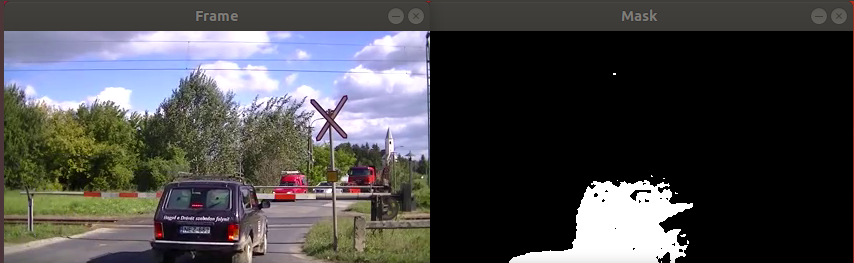
\includegraphics[width=0.32\textwidth]{Figures/R_scale50.jpg}
    }
\end{figure*}
As we see, as $R_{scale}$ grows the tree leaves that are waved by the wind are not detected
anymore as foreground but also a part of the car is lost.

\subsection*{alpha}
From eq ?????????? we see that alpha tells how much to weight the image gradients
with respect to the image values in the distance computation.
\begin{figure}[!t]
    \centering
    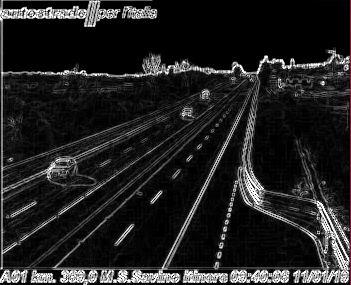
\includegraphics[width=0.45\textwidth]{Figures/gradients.jpg}
    \caption{Gradients}
    \label{fig:gradients}
\end{figure}
As we see, the image gradients give a good cue to distinguish the street from the cars
(image absolute values are not, since many cars have almost the same color of the
street). So alpha should be set high, in order to take into consideration this fact.
But notice that setting too high will lead to noisy masks, especially with noisy
videos that have small variations of the gradient from frame to frame.
\begin{figure*}[!t]
    \centering
    \subfloat[][$\alpha$ = 0]{
        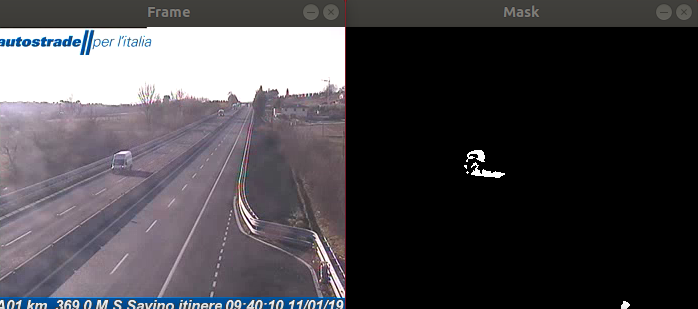
\includegraphics[width=0.32\textwidth]{Figures/alpha0.jpg}
    }
    \subfloat[][$\alpha$ = 10]{
        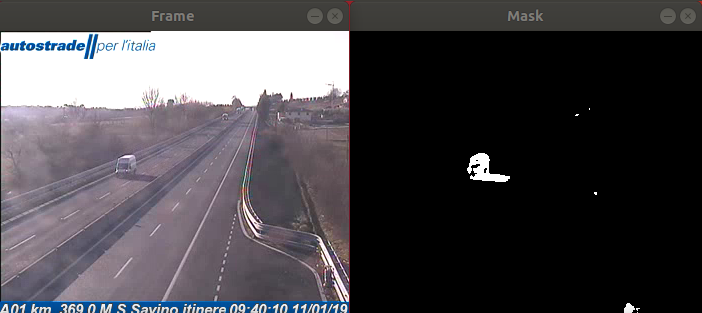
\includegraphics[width=0.32\textwidth]{Figures/alpha10.jpg}
    }
    \subfloat[][$\alpha$ = 20]{
        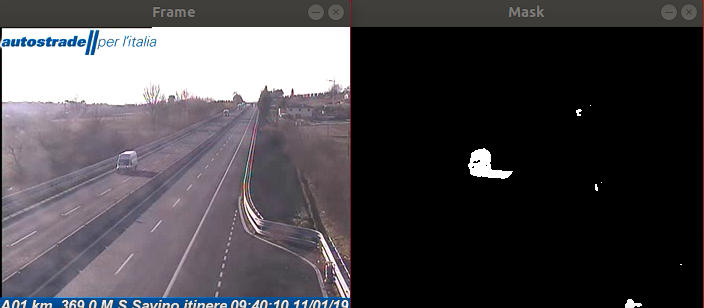
\includegraphics[width=0.32\textwidth]{Figures/alpha20.jpg}
    }
    \subfloat[][$\alpha$ = 50]{
        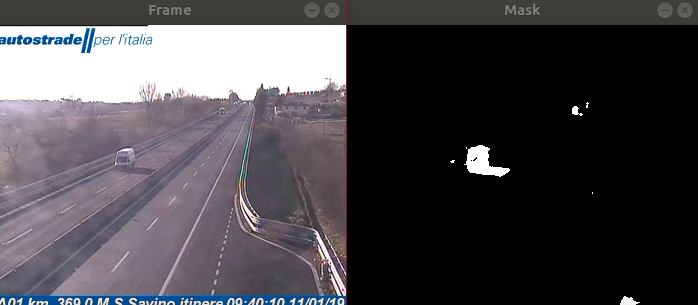
\includegraphics[width=0.32\textwidth]{Figures/alpha50.jpg}
    }
\end{figure*}




\section*{Conclusion}


